\documentclass[10pt,a4paper]{article}
\usepackage[utf8]{inputenc}
\usepackage{amsmath}
\usepackage{amsfonts}
\usepackage{amssymb}
\usepackage{graphicx}

\begin{document}

Na Figura~\ref{fig:matrix-similarity} é mostrado um exemplo de uma matriz de similaridade onde a intensidade do ponto($i,j$) representa similaridade entre as sentenças $i$ e $j$ e linha diagonal representa a similaridade entre as mesmas sentenças. Observa-se que a matriz é simétrica e revela quadrados ao longo da diagonal que indicam os as regiões com maior coesão léxica.




%representa a intensidade com que a i-ésima sentença é  similar a j-ésima sentença 




  %--- Figura Visão Geral ---
  \begin{figure}[!h]
	  \centering
	  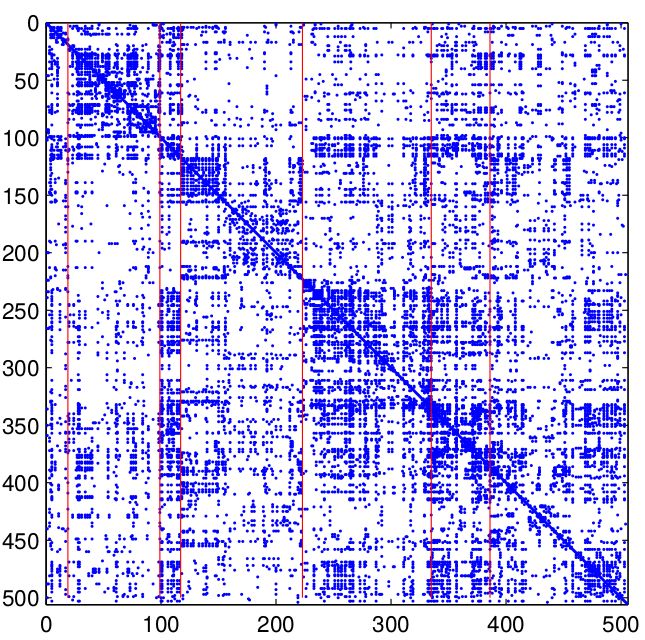
\includegraphics[width=1\textwidth]{c99.png}
	  \caption{\textit{DotPlot} da similaridade entre sentenças onde as linha verticais representam segmentos reais.}
	  \label{fig:matrix-similarity}
  \end{figure}


%%%%%%%%%%%%%%%%%%%%%%%
% - Falar do esquema de ranking;
% - Imagem com os passos e máscara 3x3;


O processo de intentificação dos limites é baseado no método DotPloting~\cite{Reynar}. Um segmento é representado por duas sentenças $i$ e $j$ que representam uma região quadrada ao londo da diagonal da matriz de similaridades. 


%%%%%%%%%%%%%%

Seja $s_{i,j}$ a somatória dos \textit{rakings} do segmento que inicia na sentença $i$ e termina na sentença $j$ e $a_{i,j}$ sua área interior. Seja $B = \{b1,...,b_m\}$ a lista de $m$ segmentos.


A medida de densidade D é dada por 

\begin{equation}
D = 
\end{equation}



onde $s_k$  $a_k$ são a somatória dos valores dos rankings e a área de um segmento $k$ em $B$.


%%%%%%%%%%%%%%


\end{document}